\documentclass[11pt]{article}
\usepackage{geometry}                
\geometry{letterpaper}                   

\usepackage{graphicx}
\usepackage{amssymb}
\usepackage{epstopdf}
\usepackage{natbib}
\usepackage{amssymb, amsmath}
\DeclareGraphicsRule{.tif}{png}{.png}{`convert #1 `dirname #1`/`basename #1 .tif`.png}

%\title{Title}
%\author{Name 1, Name 2}
%\date{date} 

\begin{document}



\thispagestyle{empty}

\begin{center}

\includegraphics[width=5cm]{ETHlogo.eps}

\bigskip


\bigskip


\bigskip


\LARGE{ 	Lecture with Computer Exercises:\\ }
\LARGE{ Modelling and Simulating Social Systems with MATLAB\\}

\bigskip

\bigskip

\small{Project Report}\\

\bigskip

\bigskip

\bigskip

\bigskip


\begin{tabular}{|c|}
\hline
\\
\textbf{\LARGE{Insert Title Here}}\\
\textbf{\LARGE{...}}\\
\\
\hline
\end{tabular}
\bigskip

\bigskip

\bigskip

\LARGE{Name 1 \& Name 2}



\bigskip

\bigskip

\bigskip

\bigskip

\bigskip

\bigskip

\bigskip

\bigskip

Zurich\\
May 2008\\

\end{center}



\newpage

%%%%%%%%%%%%%%%%%%%%%%%%%%%%%%%%%%%%%%%%%%%%%%%%%

\newpage
\section*{Agreement for free-download}
\bigskip


\bigskip


\large We hereby agree to make our source code for this project freely available for download from the web pages of the SOMS chair. Furthermore, we assure that all source code is written by ourselves and is not violating any copyright restrictions.
Several external packages are used that are freely available at Matlab FileExchange under a BSU license. 
\begin{center}

\bigskip


\bigskip


\begin{tabular}{@{}p{3.3cm}@{}p{6cm}@{}@{}p{6cm}@{}}
\begin{minipage}{3cm}

\end{minipage}
&
\begin{minipage}{6cm}
\vspace{2mm} \large Fabio Crameri

 %\vspace{\baselineskip}

\end{minipage}
&
\begin{minipage}{6cm}

\vspace{2mm} \large Marcel Thielmann

\end{minipage}
\end{tabular}


\end{center}
\newpage

%%%%%%%%%%%%%%%%%%%%%%%%%%%%%%%%%%%%%%%



% IMPORTANT
% you MUST include the ETH declaration of originality here; it is available for download on the course website or at http://www.ethz.ch/faculty/exams/plagiarism/index_EN; it can be printed as pdf and should be filled out in handwriting


%%%%%%%%%% Table of content %%%%%%%%%%%%%%%%%

\tableofcontents

\newpage

%%%%%%%%%%%%%%%%%%%%%%%%%%%%%%%%%%%%%%%



\section{Abstract}

Hei M\"ase, we should first define what we mean by social and physical forces. I'm not sure if there is something like social forces between an agent and a wall. I mean normally there is not...

I don't know how to make bold characters

\section{Individual contributions}

Fabio: 376 bugs

\section{Introduction and Motivations}

\section{Description of the Model}

\subsection{Agent}
\subsubsection{Psychological forces}

\subsubsection{Physical forces}


\subsection{Walls}

\subsubsection{Psychological forces}

The psychological repulsive force defined here for the walls/buildings can be written in mathematical terms as

\begin{equation}
	{f_{iWS}} = \left\{ {{A_i}\exp \left[ {\frac{{\left( {{r_i} - {d_{iW}}} \right)}}{{{B_i}}}} \right]} \right\}{n_{iW}} ,
	\label{eq:fiWS}
\end{equation}

where $A_i$ and $B_i$ are constants, $n_{iW}$ is the normalized vector pointing from the pedestrian to the wall, $d_{iW}$ is the distance in between and $r_i$ is the size (i.e. radius) of the pedestrian (Helbing et al., 2000).

\subsubsection{Physical forces}

The physical wall forces can be divided into a normal force and a tangential force acting from the wall and written as

\begin{equation}
	{f_{iWPn}} = \left\{ {kg\left( {{r_i} - {d_{iW}}} \right)} \right\}{n_{iW}}
	\label{eq:fiWPn}
\end{equation}

and

\begin{equation}
	{f_{iWPt}} = \left\{ {\kappa g\left( {{r_i} - {d_{iW}}} \right)\left( {{v_i} \cdot {t_{iW}}} \right)} \right\}{t_{iW}} ,
	\label{eq:fiWPt}
\end{equation}

respectively. Here, the function $g$ is zero if the pedestrian does not touch the wall, $k$ and $\kappa$ are large constants and $(v_i \cdot t_{iW})$ is the tangential velocity difference.

The total repulsive force from the architecture can then be written as

\begin{equation}
	{f_{iW}} = {f_{iWS}} + {f_{iWPn}} - {f_{iWPt}} .
	\label{eq:fiW}
\end{equation}



\subsection{Exits}

The attractive forces ($f_{iAS}$) in this work are defined in two different ways. For the simple models we use a constant force acting straight towards the attractor, neglecting obstacles in between. A more elaborated and also a more nature like formulation is used later on. It takes into account, that the pedestrians know the shortest path towards the attractive source (e.g. an exit) around any obstacle.


\subsection{Flood}

\subsection{Topography}

\subsection{Walking speed}



\section{Implementation}

This section is meant to both give an overview of the methods used in this code as well as to provide a documentation of the code. Therefore, some details are mentioned here that might not be crucial for any code that simulates pedestrian dynamics, but are needed in our implementation. 

\subsection{Initialization of Buildings and Agents}

\subsection{Agents}

\subsubsection{Agent forces}


\subsection{Architecture}

\subsubsection{Repulsive walls}

Eq. \eqref{eq:fiWS} can be rewritten as

\begin{equation}
	{f_{iWS}} = \left\{ {{A_i}\left( {\exp \left[ {\frac{{ - {d_{iW}}}}{{{B_i}}}} \right] \cdot \exp \left[ {\frac{{{r_i}}}{{{B_i}}}} \right]} \right)} \right\}{n_{iW}}
	\label{eq:fiWS2}
\end{equation}

\subsubsection{Exit forces}


\subsection{Walking speed}

\subsection{Flooding}



\section{Simulation Results and Discussion}

\subsection{Simple evacuation bottleneck: One exit}

\subsubsection{Direct exit force}

The simplest version of our code has one exit (Fig. \ref{fig:test1}). The attractive force on the agents is defined to be linear towards the exit, thereby neglecting obstacles in between. The agents will not move towards an opening in an obstacle but toward the exit itself. Moreover, this formulation inhibits the agents of running around a bigger obstacle. This is a strong simplification but suitable to test the code.
The behavior of the agents towards the repulsive walls and towards each other is satisfactory.

\begin{figure}
	\begin{center}
	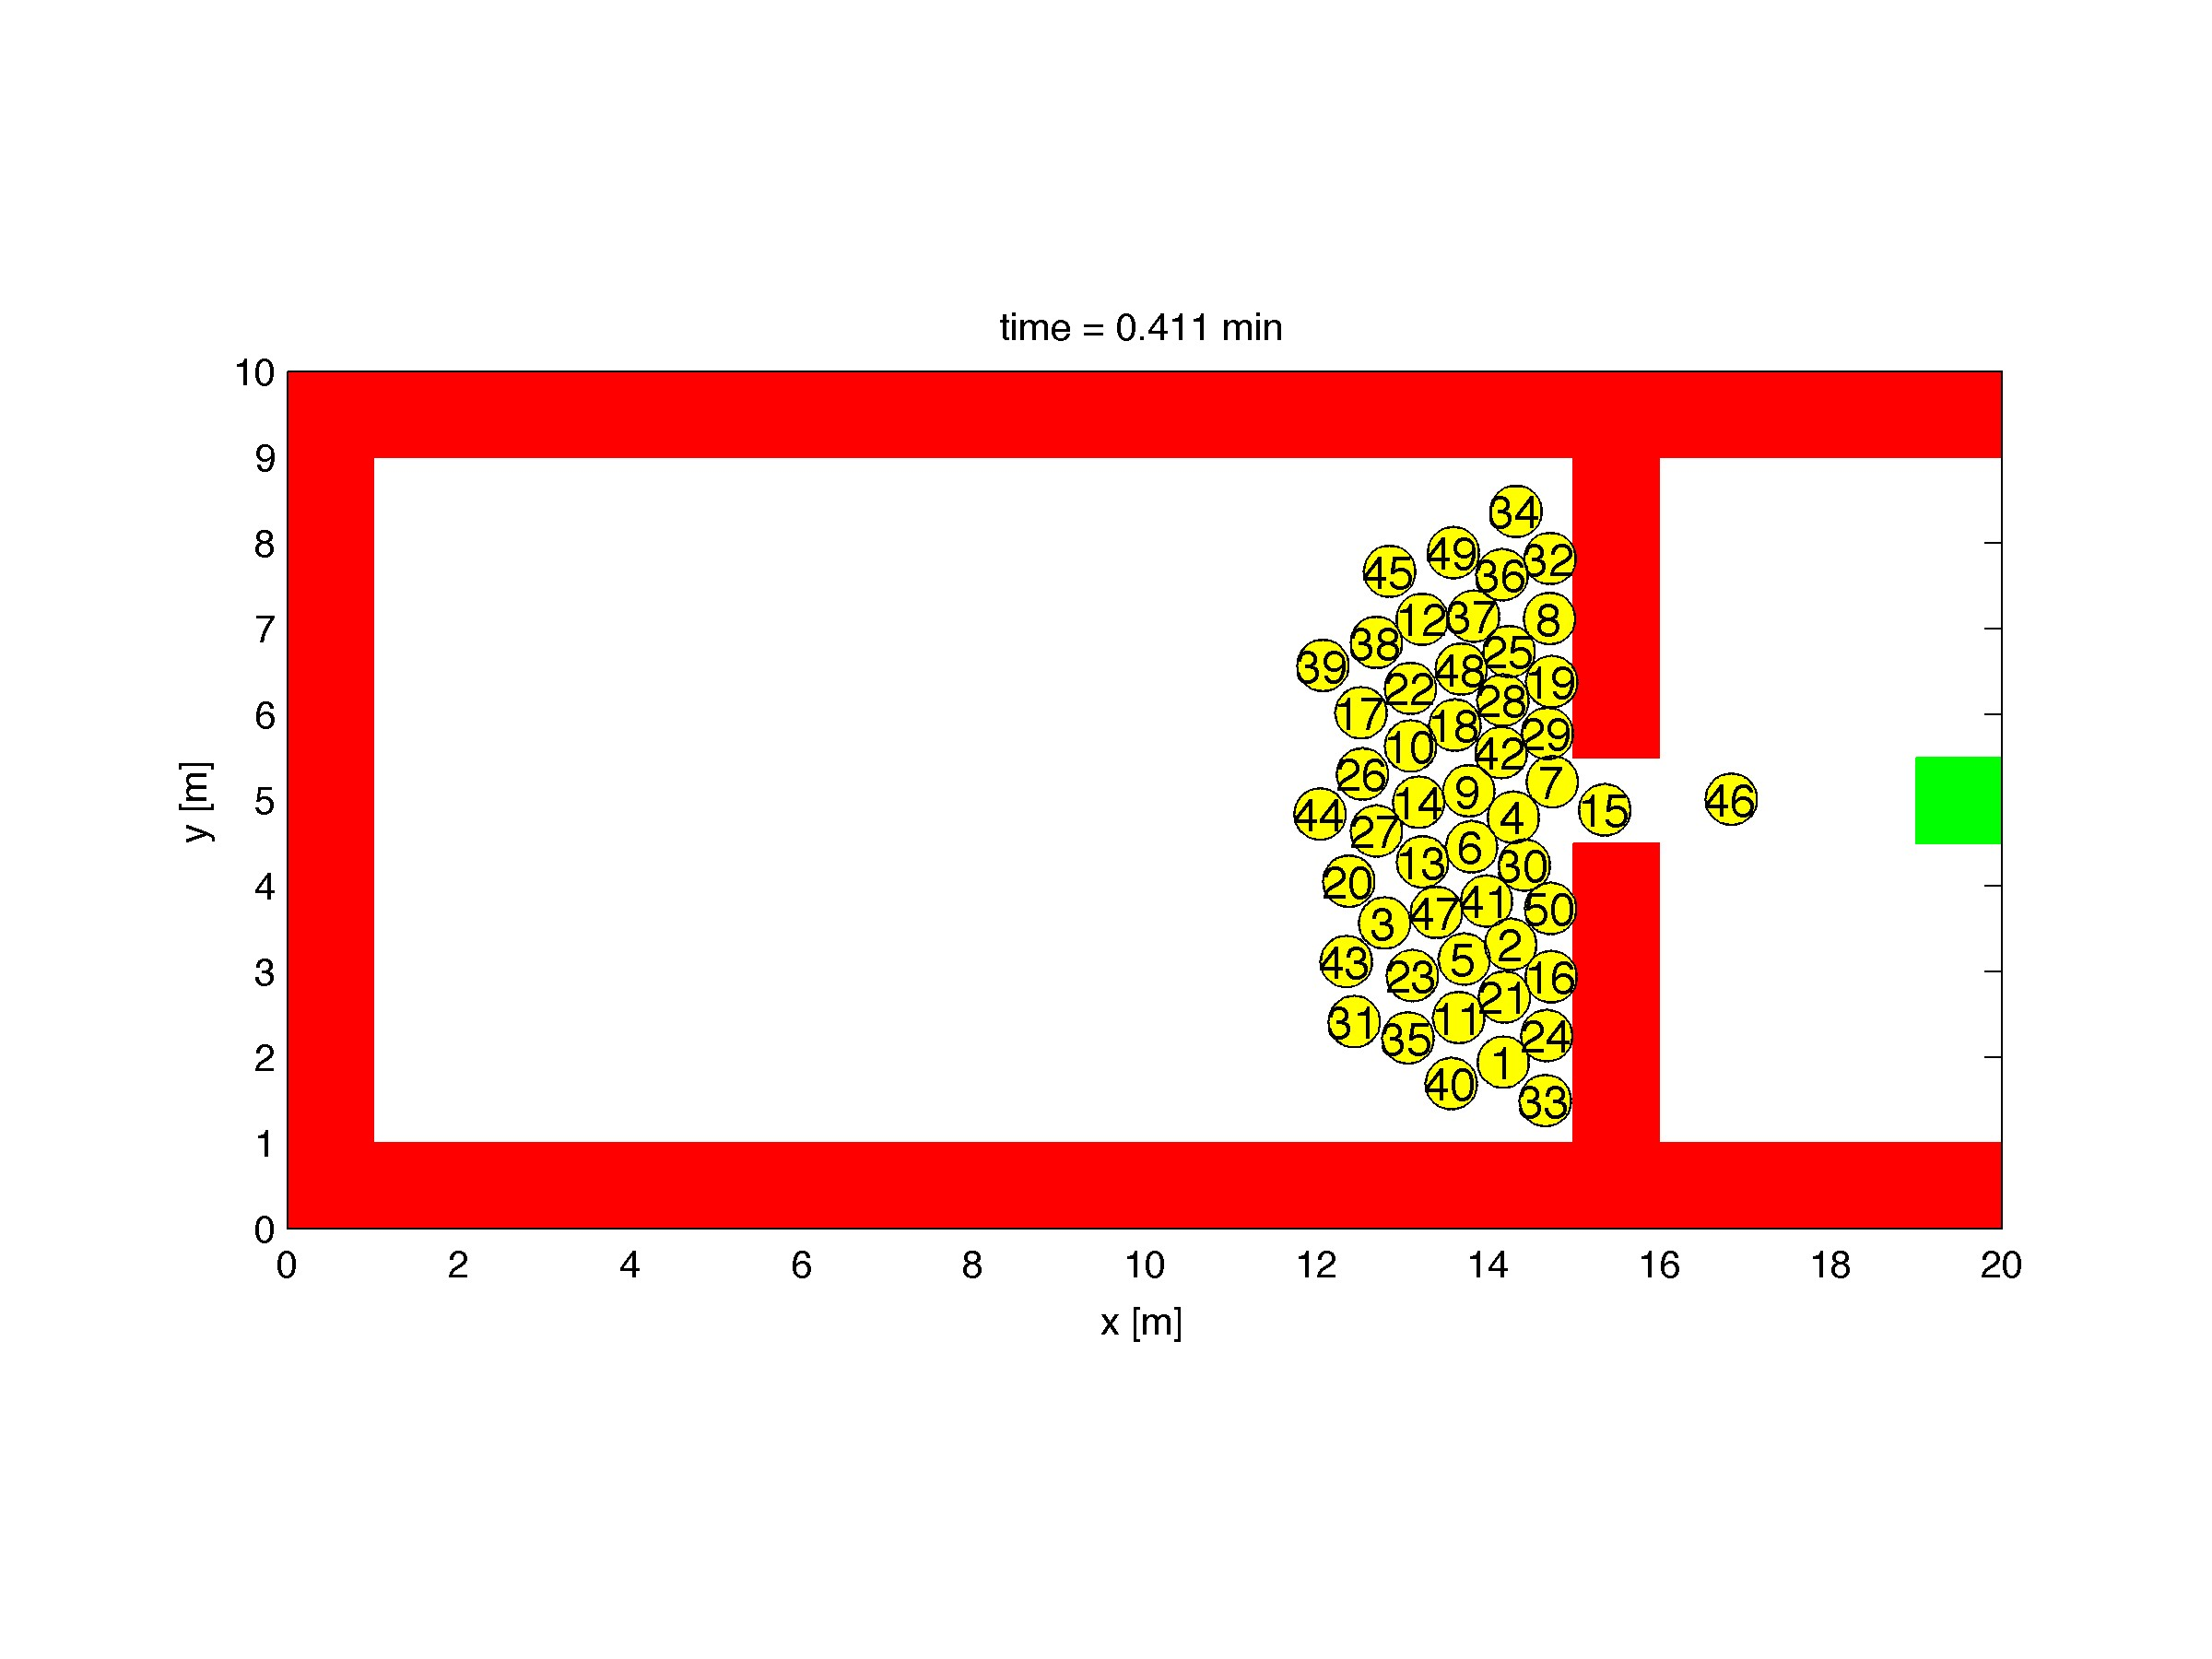
\includegraphics[width=16cm]{figures/test1000493.jpg}
	\caption{Simple simulation of an evacuation bottleneck. Agents (yellow) try to exit a room surrounded by repulsive walls (red) with an 1 m-wide door towards an attractive exit (green).}
	\label{fig:test1}
	\end{center}
\end{figure}

\subsubsection{Shortest path formulation}

\subsection{Simple evacuation bottleneck: Two exits}
\subsection{Evacuation through a road network}
\subsection{Evacuation through a road network with topography and flooding}
\subsection{Evacuation of a beach in the case of a tsunami event}

\section{Summary and Outlook}

Christmas Tree!

\section{References}

- Helbing 2000




\end{document}  



 
